
%\documentclass[11pt,a4j,ascmac]{jarticle}
\documentclass[11pt,a4j,ascmac]{jsarticle}
\usepackage{epsf}
\usepackage[dvips]{graphicx}
\usepackage{here} %記述した場所に図を出力できるパッケージ \begin{figure}[H]

\setlength{\textheight}{25cm}
\setlength{\textwidth}{16cm}
\setlength{\topmargin}{-2.5cm}
\setlength{\oddsidemargin}{0mm}
\setlength{\parindent}{0pt}
\setlength{\parskip}{3mm}

%---------------------------------------------------------------------------------------------------------------------------------------------------------

\title{第10月 進捗確認会報告資料\\
変形ARマーカの推定}

\author{ER17076 安井 理}
\date{2020年 11月 7日}
\begin{document}
\maketitle
\section{はじめに}
 10月の進捗報告を記す.
 キャッシュレス決済や物品管理,広告,ロボットの認識機能等の分野で QR コードや AR マーカに代表される 2 次元コードが利用されている.
2 次元コードには,数百から数千バイトの情報を埋め込むことができ,シンボルと呼ばれ特殊なパターンによって視点が変化しても高精度な検出が可能である.
さらに,2 次元コードの大きさを事前に定義すればカメラの位置・姿勢を推定することができる.
しかし,2 次元コードは平面に貼ることを前提条件としており,曲面に貼られた 2 次元コードは歪みによる見えの変化を引き起こすため,認識精度が低下する問題を抱えている.
研究テーマは,変形ARマーカの推定であり,鈴木さんの先行研究の改良を加えた,fastar-rcnnをAugumented AutencoderとSSDを組み合わせたものに変え,変形したARマーカの認識する手法を提案する.\\

 先行研究では,変形したARマーカの画像をFasterRCNN[1] により学習することで,歪みを含む画像を正確に認識し,ID,座標,大きさ,変形度合いを推定を行った.
今回行っている研究では,SSD・Augumented Autencoder[2]を用いてID,座標,大きさ,姿勢推定を,正確に行おうというものである.
推定した情報から歪みを取り除き,平面状のARマーカ画像に変換する.

%----------------------------------------------------------------------------------------------------------------------------------------------------------

\section{進捗報告}

\subsection{研究の目的}
 機械学習を用いることで変形による見え方を吸収し,歪んだARマーカを推定する.
歪んだARマーカを平面状に変換し出力する事.


%----------------------------------------------------------------------------------------------------------------------------------------------------------

\subsection{研究のイメージ}
 まず、画像をSSDへ入力し画像中のARマーカを検出(ID,位置,バウンディングボックス)
を出力図\ref{style1}に示す.

      \begin{figure}[htpp]
      \centering
      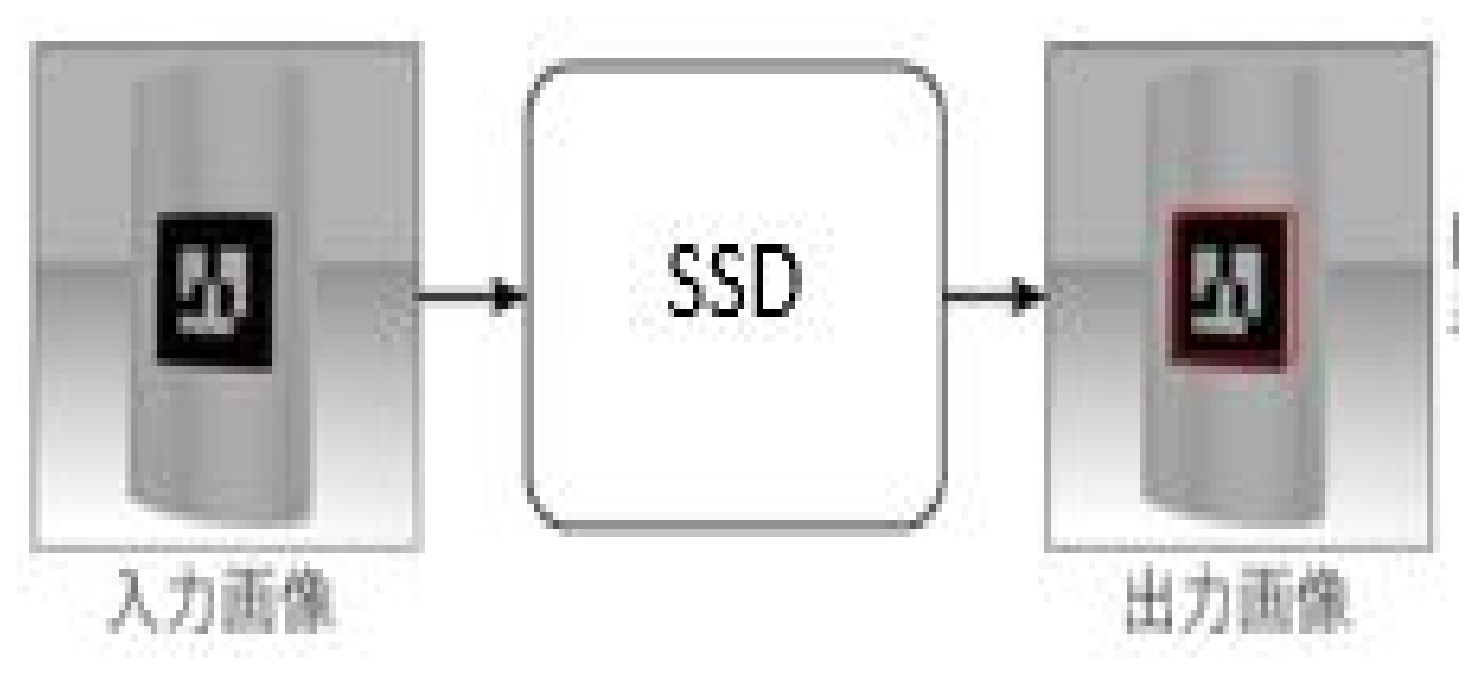
\includegraphics[width=100mm]{1.eps}
      \vspace*{40mm}
      \caption{検出.}
      \label{style1}
      \end{figure}

 この情報をもとにバウンディングボックスの画像とIDをAugumented Autencoderに入力.
ARマーカの向いてる姿勢を推定し,実際にARマーカがある位置に平面状に戻したARマーカを出力するという流れである.以下の流れを図\ref{style2}に示す.

 


      \begin{figure}[htpp]
      \centering
      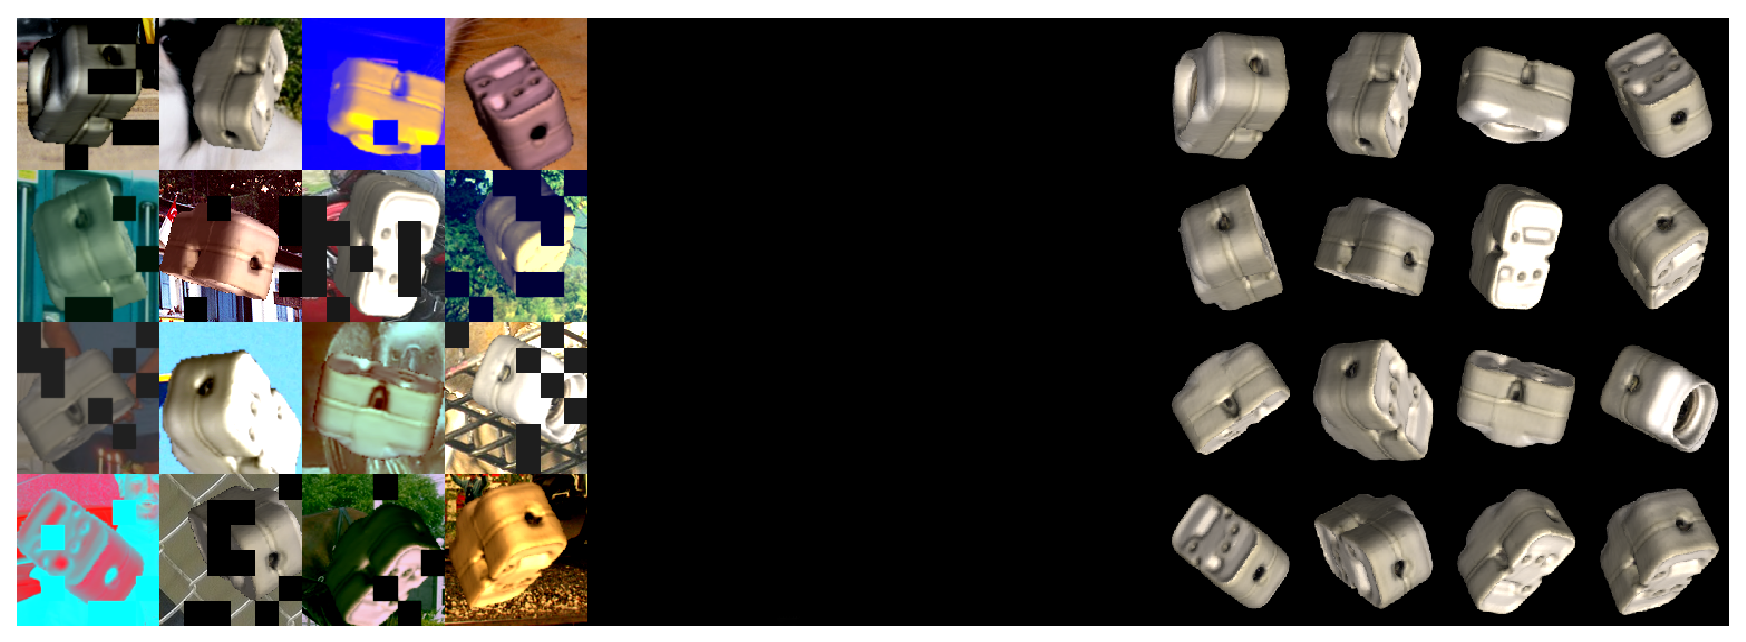
\includegraphics[width=100mm]{pic2.eps}
      \vspace*{25mm}
      \caption{全体の流れ.}
      \label{style2}
      \end{figure}



%----------------------------------------------------------------------------------------------------------------------------------------------------------

\subsection{動作確認}
 Augumented Autencoderの動作確認をまずネジのモデルを用いて行った.
目的としては,AAEを実際に自分のパソコンで実行することができるかの検証.

%----------------------------------------------------------------------------------------------------------------------------------------------------------

\subsubsection{AAEのトレーニング}
 トレーニングは,cfgファイル内のtrain temple cfg
にトレーニングを行いたいモデルと環境画像のpathを記述し,
以下のコマンドでトレーニングを開始するae train exp group/my autoencoder 
トレーニングされる画像は図\ref{style3}に示すように自動生成される。

      \begin{figure}[htpp]
      \centering
      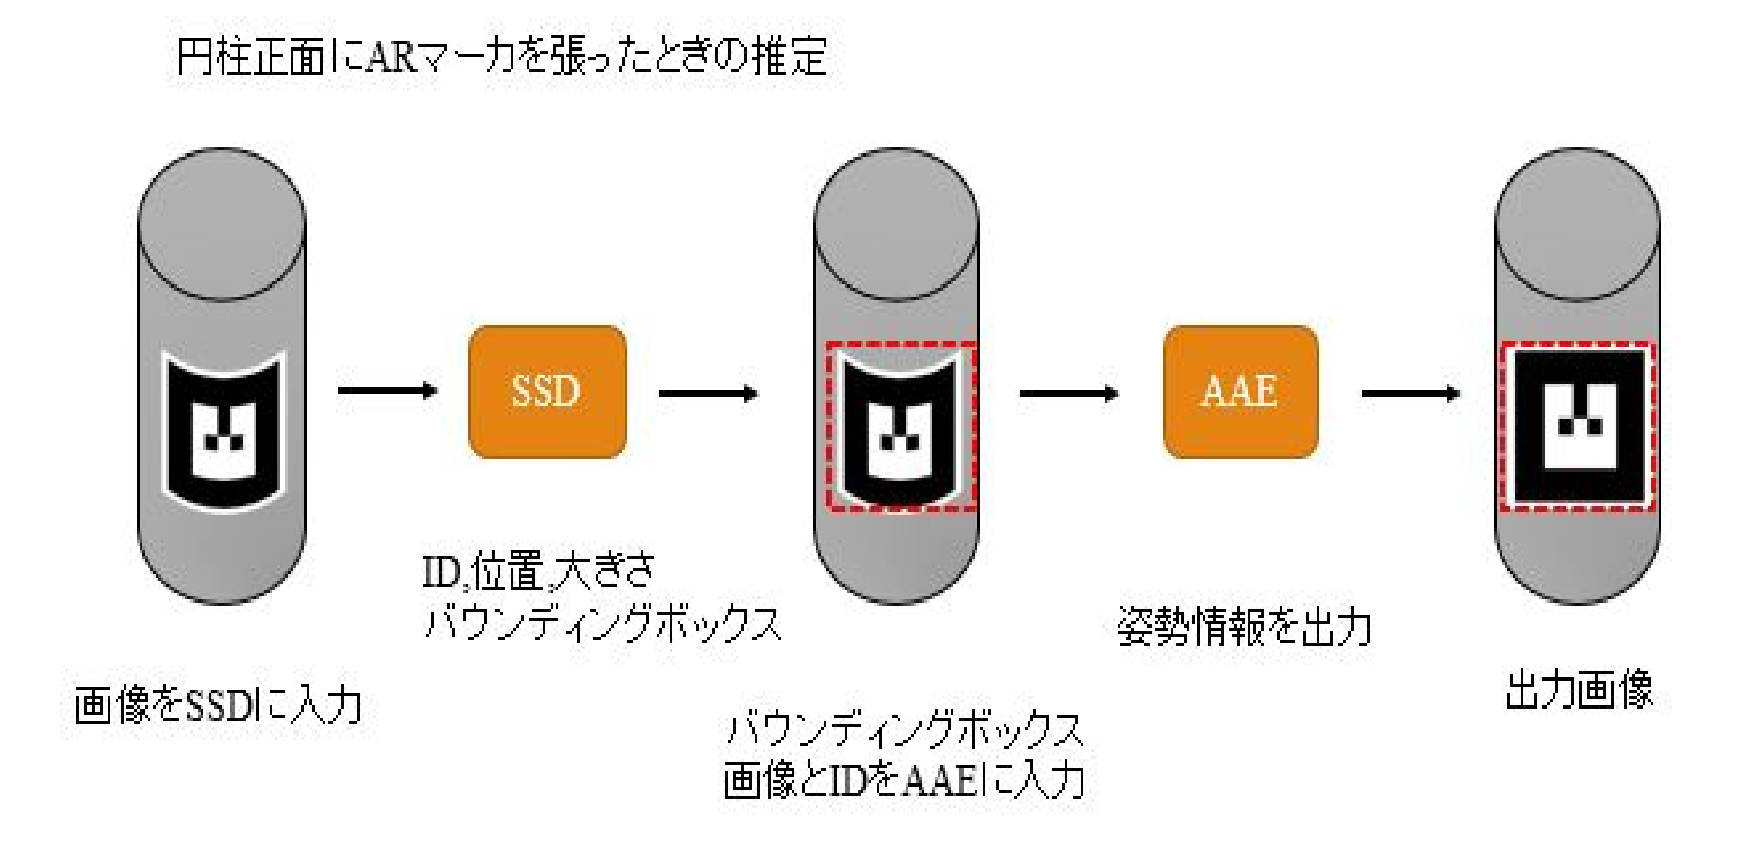
\includegraphics[width=100mm]{2.eps}
      \vspace*{25mm}
      \caption{トレーニング.}
      \label{style3}
      \end{figure}


%----------------------------------------------------------------------------------------------------------------------------------------------------------

\subsubsection{テスト}
 テストは以下のコマンドにテストしたい画像のpathを記述し実行.
python aae image.py exp group/my autoencoder -f /path/
実行結果を図\ref{style4}に示す.

     \begin{figure}[htpp]
     \centering
     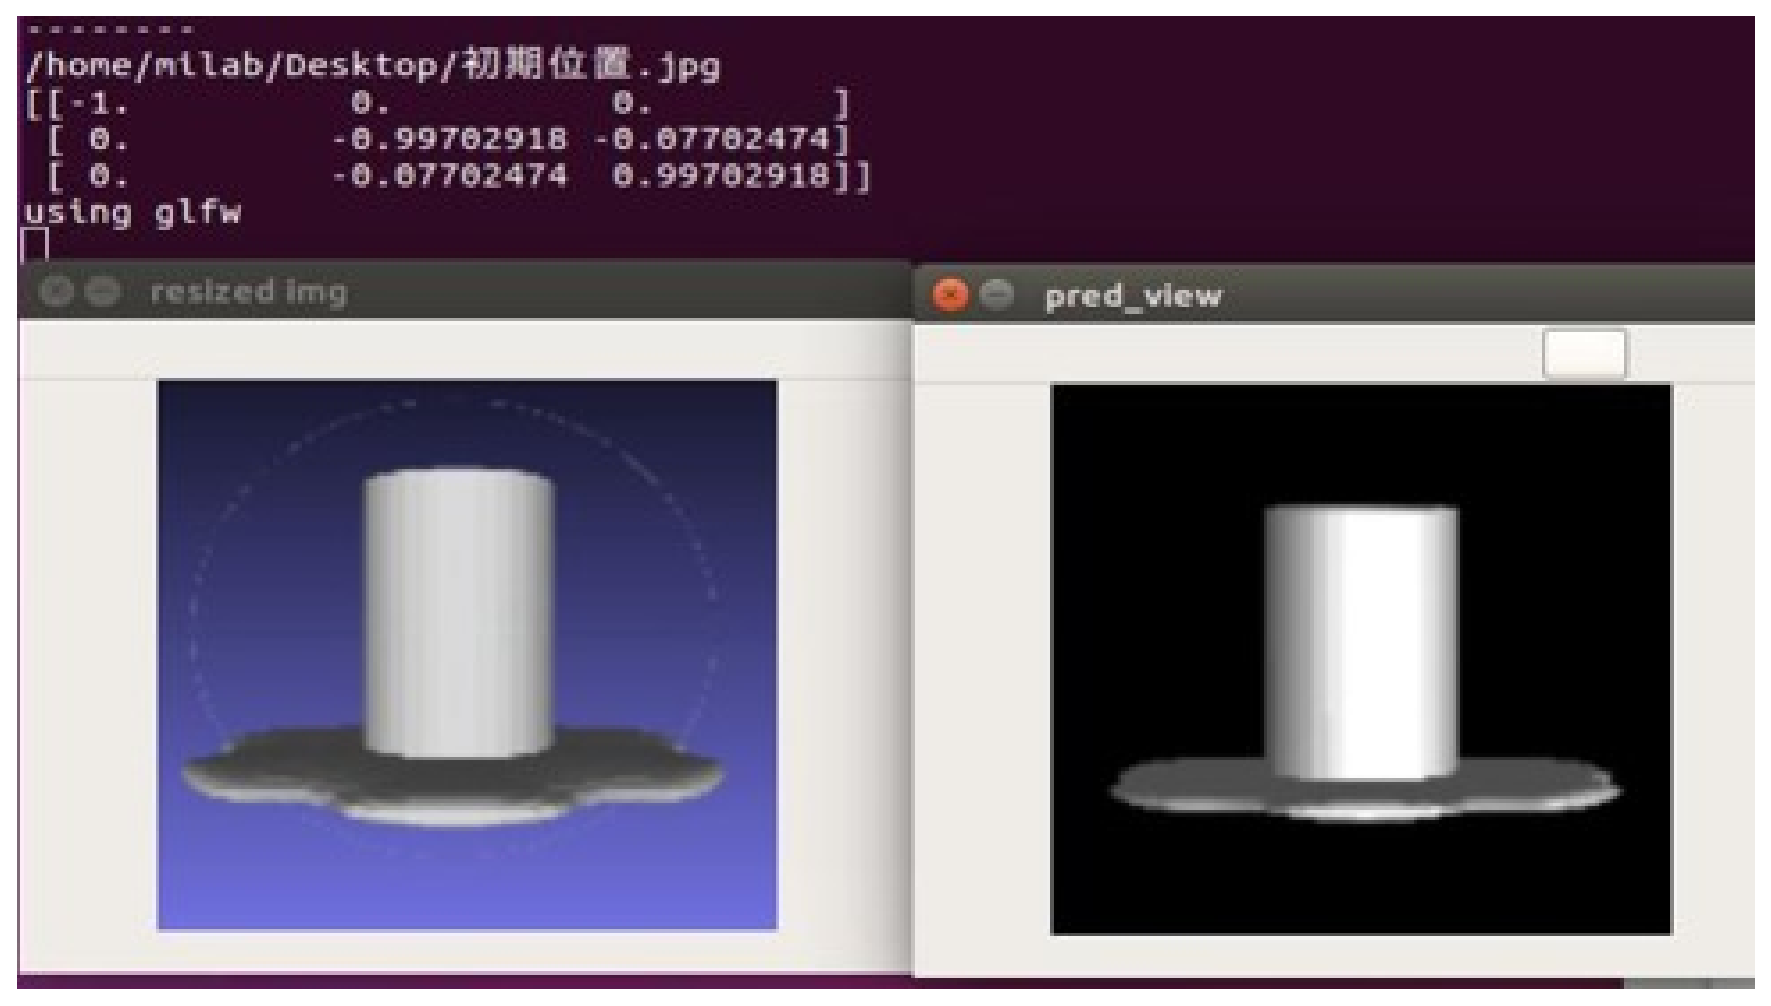
\includegraphics[width=100mm]{3.eps}
     \vspace*{25mm}
     \caption{テスト.}
     \label{style4}
     \end{figure}

複数テストを行ったがモデルがネジのため,動作確認は行えたが自分の研究への有用性はわからなかったため,自作モデルを用いて実験を行いたいと考えている.
%---------------------------------------------------------------------------------------------------------------------------------------------------------

\subsection{今後考えている実験}
 自作モデル(ARマーカ)を用いてトレーニングし自分の研究目標の一つである,AAEを用いた姿勢推定を行えるように進める.
実験で用いるテスト画像は実際にバウンディングボックスから得られるであろう画像を想定し用意し,テストを行おうと計画している




%---------------------------------------------------------------------------------------------------------------------------------------------------------
\section{おわりに}
 今回はモデルデータでのトレーニングエラーを解決するのに時間を取られてしまったため,実際の進みとしてはあまり多くないが,目標を再確認し自分のやるべきことがあいまいだったのが,少しずつ明確になってきたので,研究にもっと時間をかけて進めていきたいと考えている.自作のARマーカのモデルでトレーニングが行えたら最後の仕上げとなると考えているので,まず結果を出せるように進めていきたい

%---------------------------------------------------------------------------------------------------------------------------------------------------------

\footnotesize
\begin{thebibliography}{99}%参考文献 {数字}の中には,参考文献の数が9件以下であれば9, 99件以下であれば99
%\bibitem{キー} 参考文献(著者名,``タイトル'",雑誌名,ページ数,学会,発表年度,URL,…)
%アンダーバーの前に「\」を入力するとエラー回避できる


%山本卒業論文の参考文献

\bibitem{fasterrcnn}
S.Ren {\em et al. }: ``Faster R-CNN: Towards Real-Time Object Detectionwith Region Proposal Networks'', Proc. of NIPS,2015.


\bibitem{Implicit 3D Orientation Learning for 6D Object Detection from RGB Images}
Martin Sundermeyer Zoltan-Csaba Marton Maximilian Durner Rudolph Triebel , ''Implicit 3D Orientation Learning for 6D Object Detection from RGB Images''  2018 https://arxiv.org/pdf/1902.01275.pdf


\bibitem{VOC2007}
``The PASCAL Visual Object Classes Challenge 2007''.http://host.robots.ox.ac.uk/pascal/VOC/voc2007/index.html

\bibitem{VOC2012}
``Visual Object Classes Challenge 2012'',http://host.robots.ox.ac.uk/pascal/VOC/voc2012/index.html


\bibitem{VOC16}
Karen Simonyan,Andrew Zisserman,``VERY DEEP CONVOLUTIONAL NETWORKS FOR LARGE-SCALE IMAGE RECOGNITION'',2015


%山本卒業論文の参考文献
%\bibitem{Fitbit Charge3}
%Fitbit Charge3, https://news.mynavi.jp/article/20180821-681741/

%\bibitem{オートエンコーダとは}
%オートエンコーダとは, https://it-trend.jp/development\_tools/article/32-0024

%\bibitem{オートエンコーダについて}
%オートエンコーダについて, https://aizine.ai/auto-encoder0616/

%\bibitem{オートエンコーダ}
%Geoffrey Hinton, Ruslan Salakhutdinov, "Reducing the Dimensionality of Data with Neural Networks", 2006.

%\bibitem{RR間隔}
%RR間隔,  https://www.kango-roo.com/learning/1708/

%\bibitem{LFHF}
%LFHF, http://hclab.sakura.ne.jp/stress\_novice\_LFHF.html

\end{thebibliography}

\normalsize

\end{document}